\begin{statementbox}
\textbf{\textcolor{CStatement}{先看核心关系：点在线上，反过来也成立}}

对圆 $x^2+y^2=4$，$P(4,0)$ 对应 $l_P:x=1$；取其上的 $Q(1,\frac32)$，$Q$ 对应的 $l_Q$ 就经过 $P$。

\begin{center}
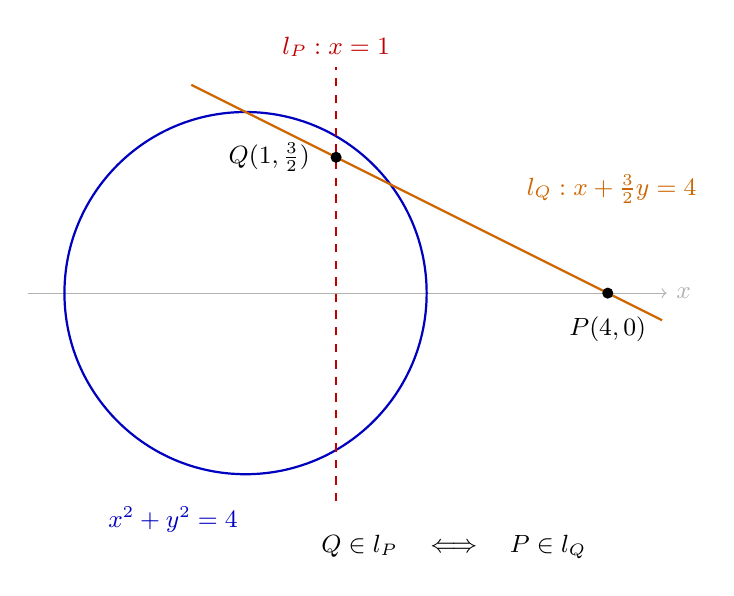
\begin{tikzpicture}[x=1.15cm,y=1.15cm,every node/.style={font=\small}]
\draw[->,gray!60] (-2.4,0)--(4.65,0) node[right] {$x$};
\draw[blue!75!black,thick] (0,0) circle (2);
\draw[red!75!black,thick,dashed] (1,-2.3)--(1,2.5);
\draw[orange!80!black,thick] (-.6,2.3)--(4.6,-.3);
\fill (4,0) circle (2pt) node[below=5pt] {$P(4,0)$};
\fill (1,1.5) circle (2pt) node[left=6pt] {$Q(1,\frac32)$};
\node[red!75!black,above] at (1,2.5) {$l_P:x=1$};
\node[orange!80!black,right] at (3,1.15) {$l_Q:x+\frac32y=4$};
\node[blue!75!black] at (-.8,-2.5) {$x^2+y^2=4$};
\node at (2.3,-2.8) {$Q\in l_P\quad\Longleftrightarrow\quad P\in l_Q$};
\end{tikzpicture}

\end{center}
图中红色虚线属于 $P$，橙色实线属于 $Q$：\textbf{看点是否落在对方的线上，而不是找点是否在自己的线上。}

\medskip
\textbf{\textcolor{CStatement}{先认清两个名称（只需要记住这两个）}}
\begin{itemize}[leftmargin=*,itemsep=0.3em]
\item \textbf{极线：} 给一个点 $P$ 配一条直线，记为 $l_P$。对圆外点，它就是从 $P$ 向圆作两条切线时，\textbf{两个切点的连线}；点在圆上时，它是该点的\textbf{切线}；点在圆内时，虽然作不出真实切线，仍可以按照\textbf{同一个方程}配出一条直线。此时只能称为“对应的极线”，不能称为真实切点的连线。
\item \textbf{极点：} 反过来，若一条直线正好是 $P$ 的极线，就称 $P$ 是这条直线的极点。简单说：\textbf{极点是点，极线是线；它们是一对对应关系。}
\end{itemize}

\medskip
\textbf{\textcolor{CStatement}{结论一：互换点的次序，关系不变}}

设 $P(x_1,y_1),Q(x_2,y_2)$ 是两个有对应极线的点，记它们的极线为 $l_P,l_Q$。那么
\[
\boxed{\ Q\in l_P\ \Longleftrightarrow\ P\in l_Q\ }.
\]
换成一句完整的话：\textbf{若 $Q$ 在 $P$ 的极线上，则 $P$ 一定在 $Q$ 的极线上；反过来也成立。} 有时把这样的两点称为“共轭点”，这只是给上面这个关系取个名字，不需要额外学习新规则。

\medskip
\par\noindent\begin{minipage}{\linewidth}
\textbf{\textcolor{CStatement}{结论二：动点在定直线上，对应的动直线过定点}}

\textbf{前提：} 已确定直线 $l$ 是某个固定点 $P$ 的极线，即 $l=l_P$。若动点 $Q$ 始终在 $l$ 上，那么
\[
\boxed{\ Q\in l_P\quad\Longrightarrow\quad P\in l_Q\ }.
\]
也就是说：$Q$ 可在 $l_P$ 上取不同位置，但每次由 $Q$ 配出的直线 $l_Q$ \textbf{都经过 $P$}。注意：\textbf{不能}对任意给定直线不加判断就声称它一定对应一个普通平面内的点。

\end{minipage}\par
\medskip
\textbf{\textcolor{CStatement}{最容易上手的圆形版本}}

对圆 $x^2+y^2=r^2\;(r>0)$：
\[
\boxed{l_P:\ x_1x+y_1y=r^2},\qquad
\boxed{P,Q\text{ 满足互换关系}\iff x_1x_2+y_1y_2=r^2}.
\]
例如 $x^2+y^2=4$，$P(4,0)$ 的极线是 $x=1$。取 $Q(1,t)$，则 $Q$ 的极线是 $x+ty=4$；把 $P(4,0)$ 代入，永远得到 $4=4$，故所有这些直线都经过 $P$。

\medskip
\textbf{\textcolor{CStatement}{其他三种常见曲线（查阅用，不要求一次背完）}}
\begin{itemize}[leftmargin=*,itemsep=0.35em]
\item 椭圆 $\dfrac{x^2}{a^2}+\dfrac{y^2}{b^2}=1\;(a>b>0)$：$\displaystyle l_P:\frac{x_1x}{a^2}+\frac{y_1y}{b^2}=1$。
\item 双曲线 $\dfrac{x^2}{A^2}-\dfrac{y^2}{B^2}=1\;(A,B>0)$：$\displaystyle l_P:\frac{x_1x}{A^2}-\frac{y_1y}{B^2}=1$。
\item 抛物线 $y^2=2px\;(p>0)$：$\displaystyle l_P:\ y_1y=p(x+x_1)$。
\end{itemize}
这三个方程都具有同一个特点：\textbf{把点 $P$ 和点 $Q$ 的坐标交换，判断式的值不变。} 因而互换结论对它们同样成立。

\medskip
\textbf{\textcolor{CStatement}{适用范围与重要例外}}

本节只讨论普通的圆、椭圆、双曲线、抛物线，不讨论方程化成两条直线等其他情况。对以原点为中心的圆、椭圆、双曲线，\textbf{原点没有这里所说的普通极线}（代入后会成为 $0=r^2$ 或 $0=1$，无法画出直线）；因此不要把中心点代入上述“点配直线”的说法。抛物线 $y^2=2px$ 则没有这个例外。
\end{statementbox}
